\subsection{Mapa cooperativo}
\textit{Mari0} es un juego open source desarrollado por la comunidad. Este juego obtuvo mucha popularidad en los años 2012 a 2015. Durante esta época se creó un foro sobre el juego donde cualquier diseñador interesado podía enviar una copia de su mapa para que el resto de los jugadores del juego pudieran valorarlo. El juego ya trae varios mapas diseñados por los creadores del juego. Todos estos mapas pueden jugarse con más de 1 jugador, pero solo es necesario 1 jugador para completarlos. Aun así, ninguno de estos es estaba completamente diseñado para un mínimo 2 o más jugadores.

En nuestro caso es necesario un mapa diseñado para 2 jugadores como mínimo. Por ello teníamos 2 opciones. La primera opción consistía en diseñar el mapa nosotros mismos. Esta tarea no es demasiado difícil, ya que el juego trae consigo un editor de niveles muy intuitivo y fácil de usar. Aun así, esta tarea no estaba prevista y aun ser sencilla, es necesario un tiempo para desarrollar y testear el mapa. La otra opción consistía en realizar una búsqueda por el foro \cite{mari0-forum} con el objetivo de encontrar algún mapa que cumpliera estas características. 

Decidimos buscar en el foro y en caso de encontrar un mapa, analizar si era viable usarlo como el mapa principal del entorno. En caso de no encontrar ninguno viable, habría que implementarlo desde 0. Para facilitar la búsqueda, se contactó con el usuario \textit{HugoBDesigner}, un diseñador muy popular de mapas de \textit{Mari0}, ya que este se dedicaba a realizar valoraciones de los mapas que le enviaban otros usuarios y colaboraba activamente con los creadores del videojuego. Este diseñador colaboró con la búsqueda aportándonos enlaces a 3 mapas cooperativos que él había jugado durante la época del 2012. De estos 3 enlaces, solo 1 permanecía activo. Este mapa llamado \textit{Bowser Cooperative Testing Initiative} fue el que usamos para como mapa principal para el entorno. El mapa puede descargarse de \cite {mari0-mapa} gracias al diseñador \textit{Pixel Worker}. 

Para comprobar que el entorno no puede ser resuelto por un solo agente usaremos la Figura \ref {fig:mapa} que es el principio del primer nivel del mapa.
\begin{figure}[ht]
    \centering
    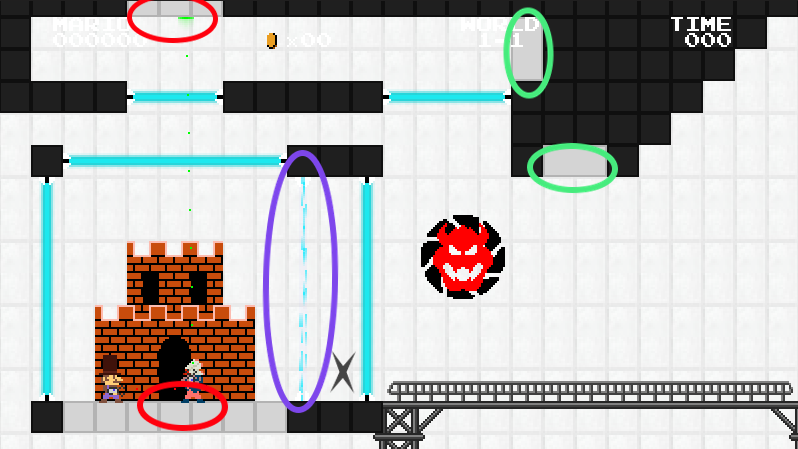
\includegraphics[width=0.9\textwidth]{img/mario-1-level.png}
    \caption{Nivel del mapa \textit{Bowser Cooperative Testing Initiative} \cite {mari0-mapa}}
    \label{fig:mapa}
\end{figure}

La forma de resolver este nivel es la siguiente:
\begin{itemize}
    \item Paso 1: En primer lugar, uno de los dos jugadores, de ahora en adelante jugador 1, debe colocar un portal en cada uno de los círculos rojos indicados en la Figura. Con este movimiento se consigue que el jugador 1 pase a la sección superior.
    \item Paso 2: El jugador 2 debe colocarse donde se encuentra la X indicada en la Figura. Desde esta posición debe disparar dos portales a los círculos verdes indicados en la Figura. Con este paso el jugador 1, que se encuentra en la sección superior, será capaz de atravesar estos portales y pasar fuera del cuadrilátero inicial.
    \item Paso 3: Una vez el jugador 1 se encuentra fuera del cuadrilátero, el jugador 2 deberá realizar las mismas acciones que el jugador 1 en el primer paso.
    \item Paso 4: Mientras eso ocurre, el jugador 1 deberá colocar sus portales donde los colocó el jugador 2 en el paso 2.
    \item Si se han realizado correctamente todos los pasos, ambos jugadores deberían haber salido del cuadrilátero inicial.
\end{itemize}

Es fácilmente visible que un solo jugador no puede completar este primer nivel. Esto se debe a que desde la sección superior es imposible colocar los portales donde debe para salir del cuadrilátero. El resto de niveles del mapa incluyen este tipo de puzzles los cuales, al igual que este, necesitan como mínimo 2 agentes para ser resueltos.